\section{Cross Correlation}
\label{sec:02_cc}

The \ac{CC} provides information about the similarity of two signals.
Thus, the delay of one signal can be detected where the \ac{CC} $r_{12}(t)$ is largest.
% -------------------------------------------------------------
In time domain, the \ac{CC} of two signals $x_0$ and $x_1$ is denoted as
\bal
    R_{x_0x_1}(t) = x_0(t) \circledast x_1(t) = \int^{+\infty}_{-\infty}x_0(\tau-t)x_1(\tau)d\tau.
\eal
Considering the frequency domain, the function can be transformed into
\bal
    \mathcal{F}[R_{12}(t)] = G_{x_0x_1}(f) = X_0^*(f)X_1(f)
\eal
with $\mathcal{F}[x_i(t)] = X_i(f)$ and $X_i^*(f)$ indicating the conjugate complex form.
% -------------------------------------------------------------
However, the finite observation time of the received signal corrupts the fourier
transform \cite{K_C_GCC}
and noise of sensors may introduce false peaks in the \ac{CC} \cite{H_B_GCC}.
% -------------------------------------------------------------
In frequency domain, the signals $x_0(t)$ and $x_1(t)$ from \cref{eq:02_signalTimeDomain}
can be expressed as
\bsub
\label{eq:02_signalFreqDomain}
\bal
    X_0(f) &= S(f) + N_0(f)\\
    X_1(f) &= \alpha S(f) e^{-j2\pi fD}+ N_1(f).
\eal \esub
% -------------------------------------------------------------
Thus, the \ac{CC} is
\bsub
\label{eq:02_Gx1x2}
\bal
    G_{x_0x_1}(f) &= \alpha |S(f)|^2 e^{-j2\pi fD} + N_0^*(f)N_1(f) + S^*(f) N_1(f) + \alpha S(f) e^{-j2\pi fD}N_0^*(f)\\
\intertext{which will be shortened as}
    G_{x_0x_1}(f) &= \alpha \phi_s(f) e^{-j2\pi fD} + \phi_n(f) + \phi_c(f) \label{eq_02_Gx1x2_simple} \\
\intertext{where}
\phi_s(f) &= |S(f)|^2 \label{eq:02_phi_s} \\
\phi_n(f) &= N_0^*(f)N_1(f) \label{eq:02_phi_n1n2} \\
\phi_c(f) &= S^*(f) N_1(f)+\alpha S(f)e^{-j2\pi fD}N_0^*(f) \label{eq:02_phi_c}.
\eal \esub
%\cite{H_B_GCC}
% -------------------------------------------------------------
Considering the ideal case where $s(t)$, $n_0(t)$ and $n_1(t)$ are uncorrelated, the terms
$\phi_c$ and $\phi_n$ disappear and the \ac{CC} results in
\bal
    R_{12}(t) = \mathcal{F}^{-1}[\alpha \phi_s(f) e^{-j2\pi fD}] = \alpha \mathcal{F}^{-1}[\phi_s(f)] \circledast \delta(t-D).
    \label{eq:02_R12_noNoise}
\eal
% \unsure[]{do I fully understand this? Is this correct?}
% This means there exists a peak at delay $D$ which is altered by the \ac{iFT}
% of the signal spectrum.
The \ac{CC} gives insight about the similarity of two signals and at peak, they
are most alike.
Thus, the shift between the zero index and the peak is the resulting delay.
% -------------------------------------------------------------
In general, $\phi_c$ and $\phi_n$ can neither be neglected nor assumed as uncorrelated to the signal \cite{H_B_prob},
so that they introduce inaccuracies and errors.
% -------------------------------------------------------------

\Cref{fig:03_ccTheory} is the outcome of two similar, but shifted sine signals with
3000\si{Hz} and normally distributed noise.
As the second signal is delayed by 10 samples, the peak can be detected where $shift = 10$.
The example signals are attached in \cref{fig:ap1_signals}.
One disadvantage of this technique is that for periodic signals the \ac{CC} also is periodic
and the peak is not always easily detectable. Noise and inaccuracies of the \ac{FFT} then
may influence the result what can make the peak unobvious \cite{L_L_GCC}.
\begin{figure}[ht]
	\centering
		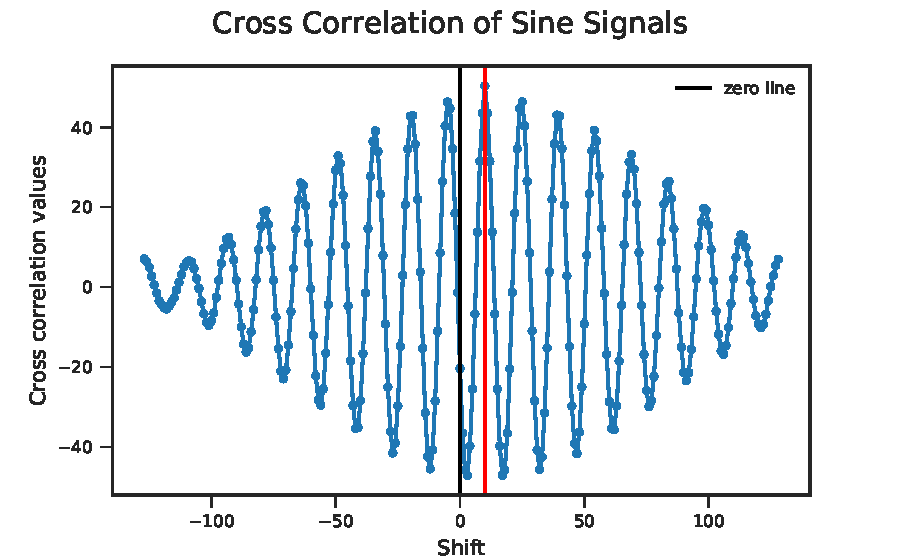
\includegraphics[width=1\columnwidth]{figures/CC_theory}
	\caption{Cross correlation of two generated sine signals with 3000Hz.}
    \label{fig:03_ccTheory}
\end{figure}
